\documentclass[final]{beamer}
\usepackage[size=custom,width=84.1,height=118.9,scale=1.35]{beamerposter}
\usepackage{booktabs,amsmath,graphicx,qrcode,ragged2e}
\usetheme{default}
\definecolor{navy}{HTML}{172554}
\definecolor{teal}{HTML}{155E75}
\definecolor{green}{HTML}{15803D}
\definecolor{orange}{HTML}{C2410C}
\definecolor{paper}{HTML}{F8FAFC}
\setbeamercolor{background canvas}{bg=paper}
\setbeamercolor{headline}{fg=white,bg=navy}
\setbeamercolor{block title}{fg=white,bg=teal}
\setbeamercolor{block body}{fg=black,bg=white}
\setbeamercolor{alertblock title}{fg=white,bg=orange}
\setbeamercolor{alertblock body}{fg=black,bg=white}
\setbeamercolor{exampleblock title}{fg=white,bg=green}
\setbeamercolor{exampleblock body}{fg=black,bg=white}
\setbeamertemplate{navigation symbols}{}
\setbeamertemplate{block begin}{
  \vskip.5ex\begin{beamercolorbox}[rounded=true,shadow=true,sep=1.5ex]{block title}
  \usebeamerfont*{block title}\insertblocktitle\end{beamercolorbox}\vspace{-.5ex}
  \begin{beamercolorbox}[rounded=true,sep=1.8ex]{block body}\justifying}
\setbeamertemplate{block end}{\end{beamercolorbox}\vskip1.4ex}
\setbeamertemplate{block alerted begin}{
  \vskip.5ex\begin{beamercolorbox}[rounded=true,shadow=true,sep=1.5ex]{alertblock title}
  \usebeamerfont*{block title}\insertblocktitle\end{beamercolorbox}\vspace{-.5ex}
  \begin{beamercolorbox}[rounded=true,sep=1.8ex]{alertblock body}\justifying}
\setbeamertemplate{block alerted end}{\end{beamercolorbox}\vskip1.4ex}
\setbeamertemplate{block example begin}{
  \vskip.5ex\begin{beamercolorbox}[rounded=true,shadow=true,sep=1.5ex]{exampleblock title}
  \usebeamerfont*{block title}\insertblocktitle\end{beamercolorbox}\vspace{-.5ex}
  \begin{beamercolorbox}[rounded=true,sep=1.8ex]{exampleblock body}\justifying}
\setbeamertemplate{block example end}{\end{beamercolorbox}\vskip1.4ex}

\begin{document}
\begin{frame}[t]
\begin{beamercolorbox}[wd=\paperwidth,sep=2.1cm,center]{headline}
{\fontsize{60}{66}\selectfont\bfseries Residual Spectral Graph Learning for\\[.3ex]
Connectivity-Loss Estimation under Multi-Edge Disruptions}\par
\vspace{1.1cm}
{\fontsize{34}{39}\selectfont\bfseries Van-Truong Le}\par
\vspace{.5cm}
{\fontsize{25}{29}\selectfont Faculty of Information Technology, University of Science,\\
Viet Nam National University Ho Chi Minh City, Viet Nam}\par
\vspace{.5cm}
{\fontsize{22}{26}\selectfont 23120181@student.hcmus.edu.vn \quad | \quad lvtruong@selab.hcmus.edu.vn}
\\[.35cm]
{\fontsize{20}{24}\selectfont ORCID: 0009-0008-7015-7392}
\end{beamercolorbox}

\vspace{1.2cm}
\begin{columns}[t,totalwidth=.96\paperwidth]
\begin{column}{.31\paperwidth}
\begin{block}{Problem and research question}
When several road links fail together, how much global connectivity is lost?
Exact recomputation is reliable but costly across many scenarios. A first-order
spectral approximation is fast and interpretable, but ignores nonlinear
interactions. We test whether a GNN should predict loss directly or learn only a
correction to the mathematical prior.
\end{block}

\begin{block}{Mathematical target}
For graph $G$ and failed edge set $S$, algebraic connectivity is the second
Laplacian eigenvalue $\lambda_2$:
\[
y(G,S)=\operatorname{clip}\!\left(1-\frac{\lambda_2(G-S)}{\lambda_2(G)},0,1\right).
\]
If $u_2$ is the Fiedler vector, first-order sensitivity gives
\[
\widehat y_{\rm spec}=\operatorname{clip}\!\left(
\frac{\sum_{(i,j)\in S}w_{ij}(u_{2,i}-u_{2,j})^2}{\lambda_2(G)},0,1\right).
\]
The residual model learns
\[
\widehat y=\operatorname{clip}(\widehat y_{\rm spec}+\tanh r_\theta,0,1).
\]
\end{block}

\begin{block}{Evaluation design}
\begin{itemize}
\item Five seeds: 11, 22, 33, 44, 55.
\item Graph-disjoint synthetic train/validation/test split.
\item Independent and spatial-cluster edge failures.
\item Zero-shot evaluation on five cached OSM networks.
\item Eight learned configurations plus the spectral baseline.
\item Paired differences and 10,000 seed-level bootstrap resamples.
\end{itemize}
\end{block}

\begin{alertblock}{Statistical guardrail}
Scenarios sharing a graph or seed are correlated. Confidence intervals resample
the five seed-level metrics - not thousands of scenario rows.
\end{alertblock}

\begin{block}{Related work and positioning}
Algebraic connectivity is a classical global robustness descriptor. Road
studies have considered random, targeted, and localized multi-link failures;
graph learning supplies nonlinear surrogates. Our contribution is the controlled
separation of a Fiedler node feature from an explicit residual prior, evaluated
with graph-disjoint splits, multi-area transfer, and seed-paired uncertainty.
\end{block}
\end{column}

\begin{column}{.32\paperwidth}
\begin{block}{Method overview}
\centering
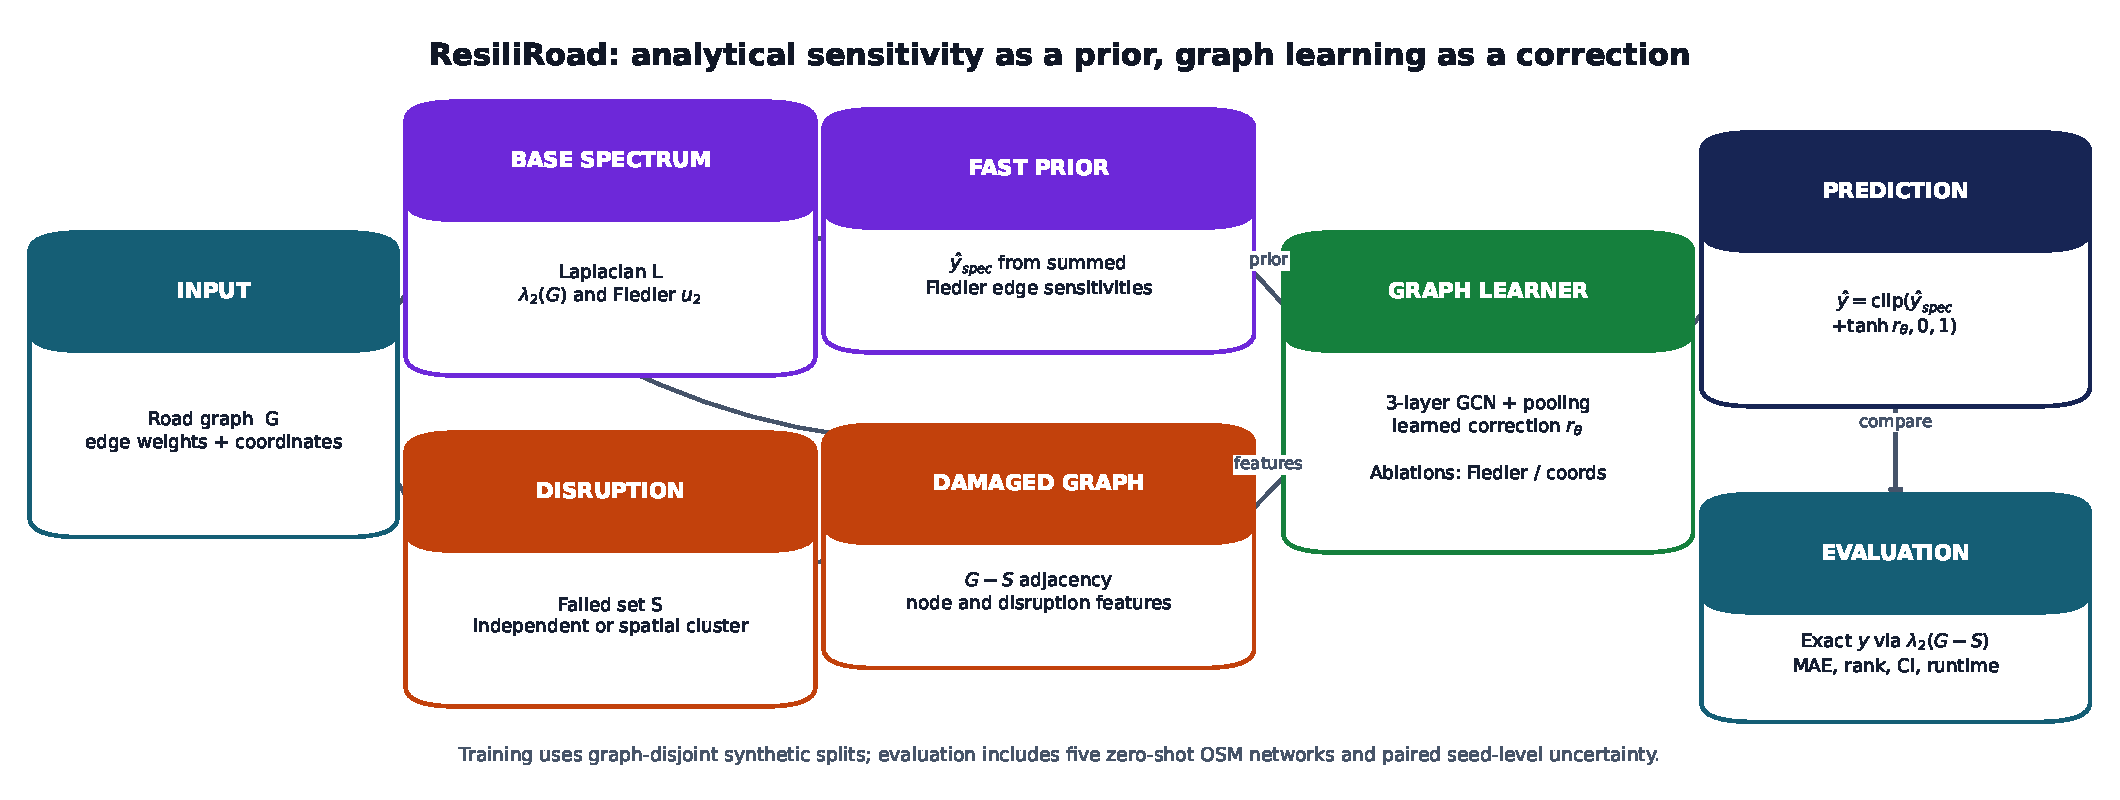
\includegraphics[width=\linewidth]{../figures/method_overview.pdf}
\end{block}

\begin{block}{Baselines and ablations}
\begin{itemize}
\item Direct GCN with all node features.
\item Direct GCN without Fiedler information or coordinates.
\item Residual GCN with the same two feature ablations.
\item Deep Sets and graph-summary MLP.
\item Exact eigendecomposition and first-order spectral estimate.
\end{itemize}
All learned models use the same graph split, optimizer, early stopping, and
80-epoch maximum.
\end{block}

\begin{block}{Five real road networks}
\centering
\begin{tabular}{lrrr}
\toprule Site & Nodes & Edges & Density\\ \midrule
HCMUS & 163 & 221 & .0167\\
VIASM & 206 & 301 & .0143\\
Da Nang & 142 & 203 & .0203\\
Can Tho & 114 & 178 & .0276\\
Da Lat & 48 & 55 & .0488\\ \bottomrule
\end{tabular}
\vspace{.7cm}

Each site contributes 100 scenarios per failure process and seed. No OSM sample
is used for training, early stopping, or model selection.
\end{block}

\begin{exampleblock}{Core finding}
The robust gain comes from the \textbf{explicit residual spectral prior}, not
from merely exposing a Fiedler node coordinate. Feature-ablation intervals cross
zero, so individual feature necessity is not claimed.
\end{exampleblock}

\begin{block}{Reproducibility}
CPU-only environment and library versions are recorded. Cached GraphML avoids
future OSM drift. One script regenerates all five seeds, bootstrap summaries,
figures, and the paper. Raw predictions are regenerable and excluded from Git to
keep the repository compact.
\end{block}
\end{column}

\begin{column}{.31\paperwidth}
\begin{block}{Zero-shot OSM results}
\centering
\begin{tabular}{lrr}
\toprule & Independent & Spatial cluster\\
Method & MAE & MAE\\ \midrule
Spectral & .502 & .650\\
Summary MLP & .281 & .347\\
Deep Sets & .114 & .143\\
Direct GCN & .106 & .102\\
\textbf{Residual GCN} & \textbf{.097} & \textbf{.090}\\
\bottomrule
\end{tabular}
\vspace{.9cm}

Paired residual improvement over direct GCN:
\begin{itemize}
\item Independent: \textbf{0.0085} [0.0039, 0.0131].
\item Spatial: \textbf{0.0121} [0.0026, 0.0247].
\end{itemize}
\end{block}

\begin{block}{Spatial-disruption comparison}
\centering
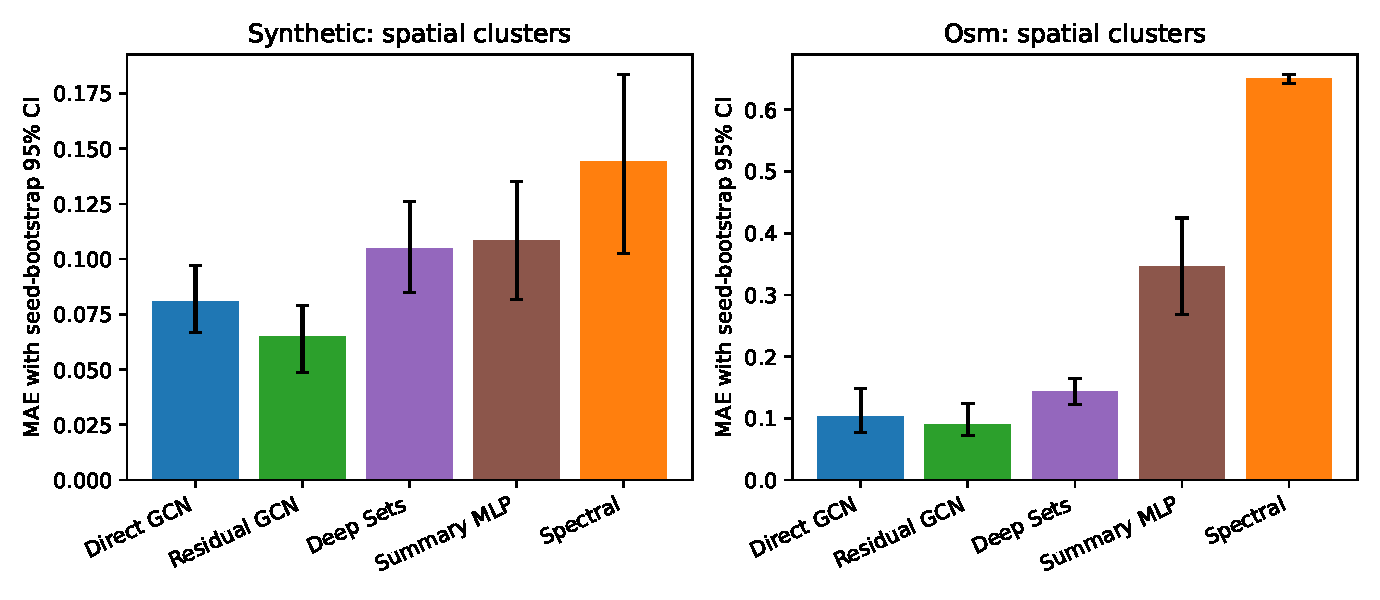
\includegraphics[width=.97\linewidth]{../outputs/paper_summary/paper_primary_results.pdf}
\end{block}

\begin{block}{Runtime on CPU}
\centering
\begin{tabular}{lr}
\toprule Method & ms/scenario\\ \midrule
Exact eigendecomposition & 5.094\\
Spectral first order & 0.018\\
Summary MLP & 0.442\\
Deep Sets & 0.430\\
Direct GCN & 0.502\\
Residual GCN & 0.674\\ \bottomrule
\end{tabular}

\vspace{.7cm}
Residual inference is about \textbf{7.6x faster} than exact recomputation on the
evaluated small OSM graphs. No GPU was used.
\end{block}

\begin{alertblock}{Where does it fail?}
Residual MAE rises from .070 on connected damaged graphs to .112 after
disconnection. Da Lat is hardest (.189 MAE), showing that density alone does not
explain transfer error. No scenario clipped the spectral estimate at one.
\end{alertblock}

\begin{block}{Takeaway, limitations, and code}
Residual spectral learning consistently improves direct regression across both
failure processes and both domains. The result concerns structural connectivity,
not flood risk, traffic demand, capacity, or recovery.

\vspace{1cm}
\begin{columns}[c]
\begin{column}{.68\linewidth}
\textbf{Paper, code, cached OSM, and reproducibility scripts:}\\[.4cm]
\url{github.com/lee-vtruong/ResiliRoad}
\end{column}
\begin{column}{.26\linewidth}
\centering\qrcode[height=5.5cm]{https://github.com/lee-vtruong/ResiliRoad}
\end{column}
\end{columns}
\end{block}
\end{column}
\end{columns}

\vfill
\begin{beamercolorbox}[wd=\paperwidth,sep=.8cm,center]{headline}
{\fontsize{20}{24}\selectfont VMS60 Poster Session - Some Topics in Modern Mathematics - VIASM, Hanoi - 4--5 December 2026}
\end{beamercolorbox}
\end{frame}
\end{document}
